\chapter{Análisis de Requisitos}
En este capítulo se detallan los requerimientos funcionales y no funcionales, de los cuales se identifican actores y casos de uso. Posteriormente, se realiza un mapeo de requerimientos a casos de uso para confirmar que se cubren todos los requerimientos con los casos de uso. Finalmente, se obtiene el modelo del dominio correspondiente.
\section{Requerimientos Funcionales}
\begin{itemize}
    \item Gestionar un conjunto de lugares.
    \item Gestionar un conjunto de cámaras de seguridad, cada una con una interfaz IP y asociada a un lugar.
    \item Gestionar placas, asociadas a códigos administrativos de los propietarios proporcionados por la institución en cuestión.
    \item Reconocer y traducir una placa vehicular. 
    \item Registrar los reconocimientos erróneos.
    \item Buscar asociación entre una placa vehicular y un código administrativo de un propietario, distinguiendo entre visitante o registrado.
    \item Registrar foto, número de placa, lugar, fecha y hora y código administrativo del propietario, asociados a un reconocimiento de una placa vehicular.
    \item Filtrar los registros almacenados en base a número de placa, lugar, fecha y hora y, código administrativo de un propietario.
    \item Generar reportes de cantidad de placas por lugares.
    \item Generar reportes de cantidad de placas de visitas contra cantidad de placas “registradas” o asociadas a un código administrativo.
\end{itemize}
Estos requerimientos caen fuera del alcance del prototipo, y serán postergados para una versión posterior:
\begin{itemize}
\item Generar reportes de tiempos de permanencia.
\item Llevar un monitoreo del estado del software.
\item Notificar si no se pudo conectar a alguna cámara.
\item Generar reportes de tiempos de inactividad del software.
\item Realizar un análisis forense en base a matriculas reconocidas parcialmente, donde se proporcionan las diversas posibles matriculas candidatas.
\end{itemize}


\section{Requerimientos No Funcionales}
\begin{itemize}
    \item Desarrollar la interfaz web del software.
    \item Desarrollar el software orientado a microservicios.
\end{itemize}

    
\section{Descripción de Actores}
\begin{enumerate}
    \item Gerente de Vigilancia: Se encarga del manejo del sistema. 
\end{enumerate}
\section{Identificación de Casos de Uso}
\addcontentsline{lot}{table}{Casos de Uso}
\begin{tabular}{@{} *5l @{}}    \toprule
\emph{\#CU} & \emph{Detalle CU} \\ \midrule
 1 & Gestionar Lugar \\ 
 2 & Gestionar Cámara \\ 
 3 & Gestionar Matricula \\ 
 4 & Gestionar Propietario \\ 
 5 & Gestionar Coincidencia \\ 
 6 & Gestionar Recolección \\ 
 7 & Gestionar Reconocimiento \\ 
 8 & Gestionar Reporte \\ \bottomrule
 \hline
\end{tabular}
\begin{landscape}
    \section{Mapeo de Requerimientos a Casos de Uso}
    % \addcontentsline{lot}{table}{Mapeo Requerimientos - Casos de Uso}
    
    \begin{table}[H]
        \centering
        \begin{tabular}{@{} *5l @{}} \toprule
        \emph{\#REQ} & \emph{Detalle REQ} & \emph{\#CU} & \emph{Detalle CU} \\ \midrule
         1 & Gestionar lugar & 1 & Gestionar Lugar \\ 
         2 & Gestionar cámaras & 2 & Gestionar Cámara \\ 
         3 & Gestionar matriculas & 3 & Gestionar Matricula \\ 
         4 & Gestionar códigos administrativos & 4 & Gestionar Propietario \\ 
         5 & Establecer conexión con cámara & 5 & Gestionar Coincidencia \\ 
         6 & Traducir una matricula & 8 & Gestionar Reporte \\ 
         7 & Buscar asociación entre matricula y propietario & 8 & Gestionar Reporte \\ 
         8 & Registrar coincidencia en BD & 8 & Gestionar Reporte \\ 
         9 & Filtrar Registros & 8 & Gestionar Reporte \\ 
         10 & Generar reporte de matriculas por lugares & 8 & Gestionar Reporte \\ 
         11 & Generar reporte de matriculas con propietario vs. no registradas & 8 & Gestionar Reporte \\  \bottomrule
         \hline
        \end{tabular}
            \caption{Mapeo Requerimientos - Casos de Uso}
            \label{tab:tab-mapeo}
    \end{table}
    
    % \begin{tabular}{@{} *5l @{}}    \toprule
    %     \end{tabular}
\end{landscape}

\begin{landscape}
\section{Modelo del Dominio}
    \begin{figure}[H]
        \centering
        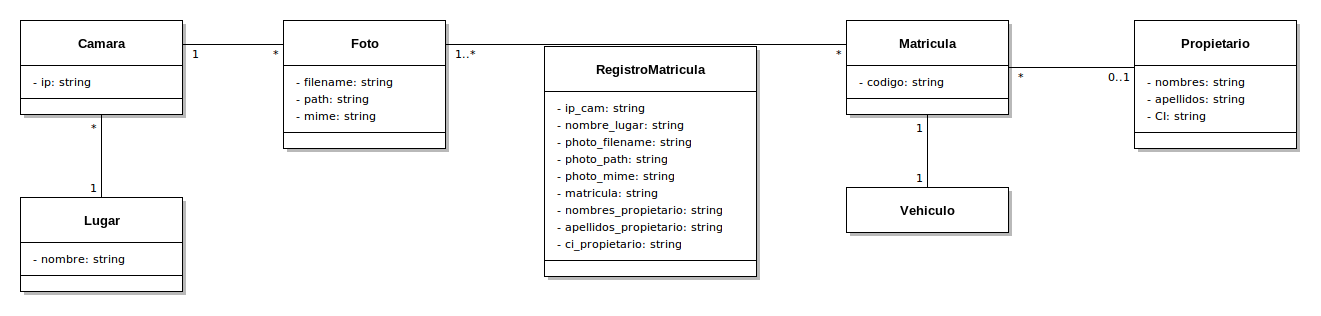
\includegraphics[width=1.3\textwidth]{DOM}
        \caption{Modelo del Dominio}
        \label{fig:DOM}
    \end{figure}
    
\end{landscape}
